
\chapter{Models and the admin site}

\section{Database setup}

Now, open up \keyword{mysite/settings.py}. It’s a normal Python module with module-level variables representing Django settings.

By default, the configuration uses SQLite.
SQLite is included in Python, so you won’t need to install anything else to support your database.
When starting your first real project, however, you may want to use a more scalable database like PostgreSQL, to avoid database-switching headaches down the road.


While you’re editing \keyword{mysite/settings.py}, set \verb|TIME_ZONE| to your time zone.
\begin{tcolorbox}
\begin{verbatim}
TIME_ZONE = 'Asia/Shanghai'
\end{verbatim}
  
\end{tcolorbox}



\section{Creating models}

In our poll app, we’ll create two models: \keyword{Question} and \keyword{Choice}.
A Question has a question and a publication date.
A Choice has two fields: the text of the choice and a vote tally.
Each Choice is associated with a Question.


These concepts are represented by Python classes.
Edit the \keyword{polls/models.py} file so it looks like this:
\lstset{language=Python}
\begin{lstlisting}
  from django.db import models


  # Create your models here.
  class Question(models.Model):
  question_text = models.CharField(max_length=200)
  pub_date = models.DateTimeField('data published')


  class Choice(models.Model):
  question = models.ForeignKey(Question, on_delete=models.CASCADE)
  choice_text = models.CharField(max_length=200)
  votes = models.IntegerField(default=0)

\end{lstlisting}


\section{Activating models}

To include the app in our project, we need a reference to its configuration class in the \verb|INSTALLED_APPS| setting.
The \keyword{PollsConfig} class is in the \keyword{polls/apps.py} file, so its dotted path is \keyword{'polls.apps.PollsConfig'}.
Edit the \keyword{mysite/settings.py} file and add that dotted path to the \verb|INSTALLED_APPS| setting.
It’ll look like this:
\begin{tcolorbox}
\begin{verbatim}
INSTALLED_APPS = [
    'polls.apps.PollsConfig',
    'django.contrib.admin',
    'django.contrib.auth',
    'django.contrib.contenttypes',
    'django.contrib.sessions',
    'django.contrib.messages',
    'django.contrib.staticfiles',
]
\end{verbatim}
\end{tcolorbox}

Now Django knows to include the \keyword{polls} app.


Three steps to make model changes:
\begin{enumerate}
\item Change your models (in \keyword{models.py})
\item Run \verb|python manager.py makemigrations| to create migrations for those changes
\item Run \verb|python manage.py migrate| to apply those changes to the database
\end{enumerate}


\section{Introducing the Django Admin}

\subsection{Creating an admin user}

\lstset{language=Sh}
\begin{lstlisting}
  python manage.py createsuperuser
\end{lstlisting}



\subsection{Make the poll app modifiable in the admin}

We need to tell the admin that \keyword{Question} objects have an admin interface.
To do this, open the \keyword{polls/admin.py} file, and edit it to look like this:

\lstset{language=Python}
\begin{lstlisting}
  from django.contrib import admin
  from .models import Question

  # Register your models here.
  admin.site.register(Question)
  
\end{lstlisting}

The registered website is shown in Figure \ref{fig:register}:
\begin{figure}[!ht]
  \centering
  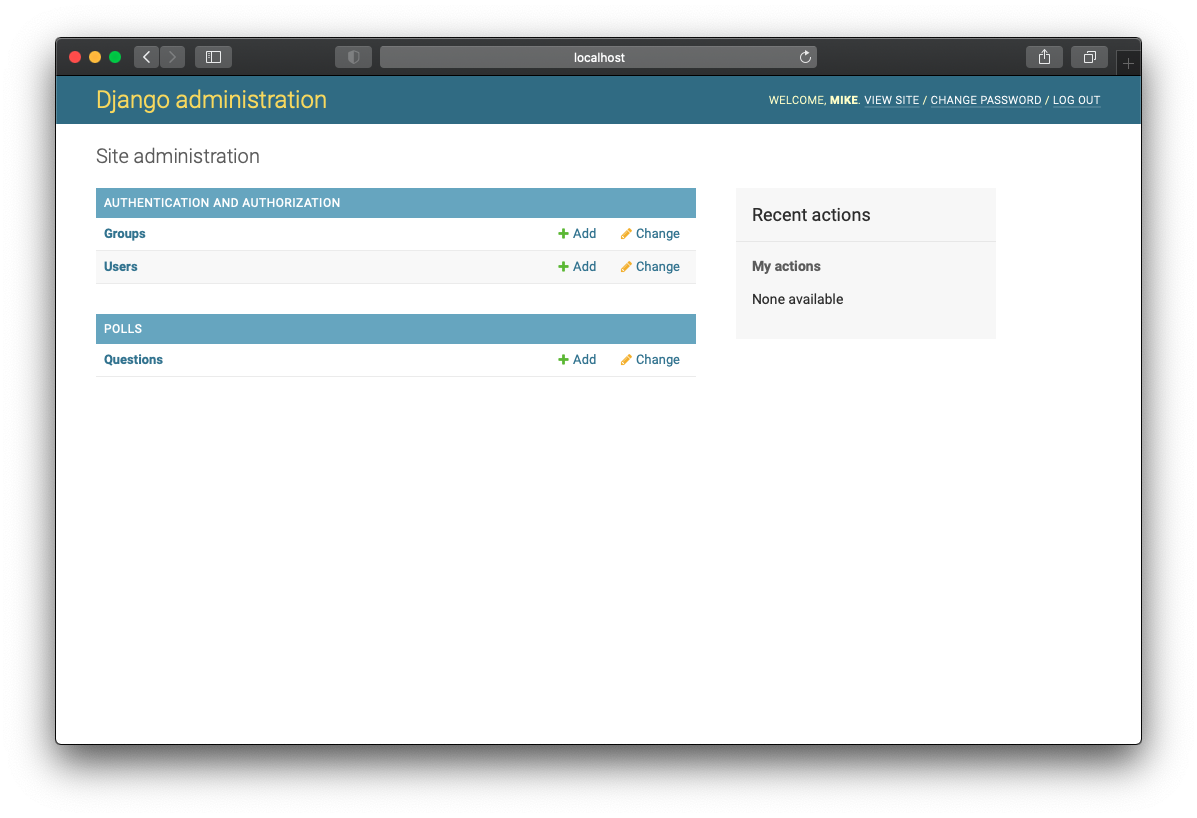
\includegraphics[width=\textwidth]{regist.png}
  \caption{Register}
  \label{fig:register}
\end{figure}


